\documentclass[]{book}
\usepackage{lmodern}
\usepackage{amssymb,amsmath}
\usepackage{ifxetex,ifluatex}
\usepackage{fixltx2e} % provides \textsubscript
\ifnum 0\ifxetex 1\fi\ifluatex 1\fi=0 % if pdftex
  \usepackage[T1]{fontenc}
  \usepackage[utf8]{inputenc}
\else % if luatex or xelatex
  \ifxetex
    \usepackage{mathspec}
  \else
    \usepackage{fontspec}
  \fi
  \defaultfontfeatures{Ligatures=TeX,Scale=MatchLowercase}
\fi
% use upquote if available, for straight quotes in verbatim environments
\IfFileExists{upquote.sty}{\usepackage{upquote}}{}
% use microtype if available
\IfFileExists{microtype.sty}{%
\usepackage{microtype}
\UseMicrotypeSet[protrusion]{basicmath} % disable protrusion for tt fonts
}{}
\usepackage[margin=1in]{geometry}
\usepackage{hyperref}
\hypersetup{unicode=true,
            pdftitle={R Advanced Spatial Lessons},
            pdfauthor={Ben Best},
            pdfborder={0 0 0},
            breaklinks=true}
\urlstyle{same}  % don't use monospace font for urls
\usepackage{color}
\usepackage{fancyvrb}
\newcommand{\VerbBar}{|}
\newcommand{\VERB}{\Verb[commandchars=\\\{\}]}
\DefineVerbatimEnvironment{Highlighting}{Verbatim}{commandchars=\\\{\}}
% Add ',fontsize=\small' for more characters per line
\usepackage{framed}
\definecolor{shadecolor}{RGB}{248,248,248}
\newenvironment{Shaded}{\begin{snugshade}}{\end{snugshade}}
\newcommand{\KeywordTok}[1]{\textcolor[rgb]{0.13,0.29,0.53}{\textbf{{#1}}}}
\newcommand{\DataTypeTok}[1]{\textcolor[rgb]{0.13,0.29,0.53}{{#1}}}
\newcommand{\DecValTok}[1]{\textcolor[rgb]{0.00,0.00,0.81}{{#1}}}
\newcommand{\BaseNTok}[1]{\textcolor[rgb]{0.00,0.00,0.81}{{#1}}}
\newcommand{\FloatTok}[1]{\textcolor[rgb]{0.00,0.00,0.81}{{#1}}}
\newcommand{\ConstantTok}[1]{\textcolor[rgb]{0.00,0.00,0.00}{{#1}}}
\newcommand{\CharTok}[1]{\textcolor[rgb]{0.31,0.60,0.02}{{#1}}}
\newcommand{\SpecialCharTok}[1]{\textcolor[rgb]{0.00,0.00,0.00}{{#1}}}
\newcommand{\StringTok}[1]{\textcolor[rgb]{0.31,0.60,0.02}{{#1}}}
\newcommand{\VerbatimStringTok}[1]{\textcolor[rgb]{0.31,0.60,0.02}{{#1}}}
\newcommand{\SpecialStringTok}[1]{\textcolor[rgb]{0.31,0.60,0.02}{{#1}}}
\newcommand{\ImportTok}[1]{{#1}}
\newcommand{\CommentTok}[1]{\textcolor[rgb]{0.56,0.35,0.01}{\textit{{#1}}}}
\newcommand{\DocumentationTok}[1]{\textcolor[rgb]{0.56,0.35,0.01}{\textbf{\textit{{#1}}}}}
\newcommand{\AnnotationTok}[1]{\textcolor[rgb]{0.56,0.35,0.01}{\textbf{\textit{{#1}}}}}
\newcommand{\CommentVarTok}[1]{\textcolor[rgb]{0.56,0.35,0.01}{\textbf{\textit{{#1}}}}}
\newcommand{\OtherTok}[1]{\textcolor[rgb]{0.56,0.35,0.01}{{#1}}}
\newcommand{\FunctionTok}[1]{\textcolor[rgb]{0.00,0.00,0.00}{{#1}}}
\newcommand{\VariableTok}[1]{\textcolor[rgb]{0.00,0.00,0.00}{{#1}}}
\newcommand{\ControlFlowTok}[1]{\textcolor[rgb]{0.13,0.29,0.53}{\textbf{{#1}}}}
\newcommand{\OperatorTok}[1]{\textcolor[rgb]{0.81,0.36,0.00}{\textbf{{#1}}}}
\newcommand{\BuiltInTok}[1]{{#1}}
\newcommand{\ExtensionTok}[1]{{#1}}
\newcommand{\PreprocessorTok}[1]{\textcolor[rgb]{0.56,0.35,0.01}{\textit{{#1}}}}
\newcommand{\AttributeTok}[1]{\textcolor[rgb]{0.77,0.63,0.00}{{#1}}}
\newcommand{\RegionMarkerTok}[1]{{#1}}
\newcommand{\InformationTok}[1]{\textcolor[rgb]{0.56,0.35,0.01}{\textbf{\textit{{#1}}}}}
\newcommand{\WarningTok}[1]{\textcolor[rgb]{0.56,0.35,0.01}{\textbf{\textit{{#1}}}}}
\newcommand{\AlertTok}[1]{\textcolor[rgb]{0.94,0.16,0.16}{{#1}}}
\newcommand{\ErrorTok}[1]{\textcolor[rgb]{0.64,0.00,0.00}{\textbf{{#1}}}}
\newcommand{\NormalTok}[1]{{#1}}
\usepackage{longtable,booktabs}
\usepackage{graphicx,grffile}
\makeatletter
\def\maxwidth{\ifdim\Gin@nat@width>\linewidth\linewidth\else\Gin@nat@width\fi}
\def\maxheight{\ifdim\Gin@nat@height>\textheight\textheight\else\Gin@nat@height\fi}
\makeatother
% Scale images if necessary, so that they will not overflow the page
% margins by default, and it is still possible to overwrite the defaults
% using explicit options in \includegraphics[width, height, ...]{}
\setkeys{Gin}{width=\maxwidth,height=\maxheight,keepaspectratio}
\IfFileExists{parskip.sty}{%
\usepackage{parskip}
}{% else
\setlength{\parindent}{0pt}
\setlength{\parskip}{6pt plus 2pt minus 1pt}
}
\setlength{\emergencystretch}{3em}  % prevent overfull lines
\providecommand{\tightlist}{%
  \setlength{\itemsep}{0pt}\setlength{\parskip}{0pt}}
\setcounter{secnumdepth}{5}
% Redefines (sub)paragraphs to behave more like sections
\ifx\paragraph\undefined\else
\let\oldparagraph\paragraph
\renewcommand{\paragraph}[1]{\oldparagraph{#1}\mbox{}}
\fi
\ifx\subparagraph\undefined\else
\let\oldsubparagraph\subparagraph
\renewcommand{\subparagraph}[1]{\oldsubparagraph{#1}\mbox{}}
\fi

%%% Use protect on footnotes to avoid problems with footnotes in titles
\let\rmarkdownfootnote\footnote%
\def\footnote{\protect\rmarkdownfootnote}

%%% Change title format to be more compact
\usepackage{titling}

% Create subtitle command for use in maketitle
\newcommand{\subtitle}[1]{
  \posttitle{
    \begin{center}\large#1\end{center}
    }
}

\setlength{\droptitle}{-2em}
  \title{R Advanced Spatial Lessons}
  \pretitle{\vspace{\droptitle}\centering\huge}
  \posttitle{\par}
  \author{Ben Best}
  \preauthor{\centering\large\emph}
  \postauthor{\par}
  \predate{\centering\large\emph}
  \postdate{\par}
  \date{2017-09-27}

\usepackage{booktabs}
\usepackage{amsthm}
\makeatletter
\def\thm@space@setup{%
  \thm@preskip=8pt plus 2pt minus 4pt
  \thm@postskip=\thm@preskip
}
\makeatother

\usepackage{amsthm}
\newtheorem{theorem}{Theorem}[chapter]
\newtheorem{lemma}{Lemma}[chapter]
\theoremstyle{definition}
\newtheorem{definition}{Definition}[chapter]
\newtheorem{corollary}{Corollary}[chapter]
\newtheorem{proposition}{Proposition}[chapter]
\theoremstyle{definition}
\newtheorem{example}{Example}[chapter]
\theoremstyle{definition}
\newtheorem{exercise}{Exercise}[chapter]
\theoremstyle{remark}
\newtheorem*{remark}{Remark}
\newtheorem*{solution}{Solution}
\begin{document}
\maketitle

{
\setcounter{tocdepth}{1}
\tableofcontents
}
\chapter*{Prerequisites}\label{prereq}
\addcontentsline{toc}{chapter}{Prerequisites}

Lessons presented here are a continuation of the
\href{http://www.datacarpentry.org/lessons/\#geospatial-data-workshop}{Geospatial
workshop using R of Data Carpentry} described more specifically for the
\href{https://jsta.github.io/2017-09-27-LBNL/}{Lawrence Berkeley
National Lab: Sep 27-28, 2017}.

This content is setup for now using
\href{http://bookdown.org/yihui/bookdown}{bookdown} (using the
\href{https://github.com/rstudio/bookdown-demo}{bookdown-demo}) for
expediency, and meant to eventually be folded into the
\href{https://github.com/swcarpentry/styles}{Software Carpentry style}.

\chapter*{Setup}\label{setup}
\addcontentsline{toc}{chapter}{Setup}

\section{Install software}\label{install-software}

This workshop will require the following software installed on your
machine:

\begin{itemize}
\tightlist
\item
  \href{http://cran.cnr.berkeley.edu/}{R}
\item
  \href{https://www.rstudio.com/products/rstudio/download/\#download}{RStudio}
\end{itemize}

Please download the appropriate stable release for your operating
system.

\section{Launch RStudio}\label{launch-rstudio}

RStudio is an integrated development environment (IDE) for editing text
in the code editor, running commands in the R console, viewing defined
objects in the workspace and past commands in the history, and viewing
plots, files and help. Here's a layout of the panes in RStudio, each of
which can have several tabs for alternate functionality:

\begin{figure}[htbp]
\centering
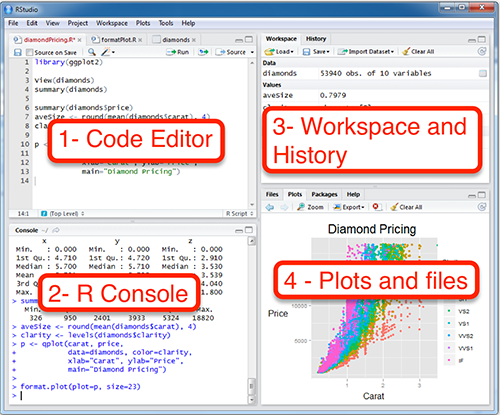
\includegraphics{figs/rstudio.png}
\caption{}
\end{figure}

Check out the Help \textgreater{} Cheatsheets \textgreater{}
\href{https://github.com/rstudio/cheatsheets/raw/master/rstudio-ide.pdf}{RStudio
IDE Cheat Sheet}.

\section{Create RStudio project}\label{create-rstudio-project}

In RStudio, please create an RStudio project (File \textgreater{} New
Project\ldots{} \textgreater{} New Directory \textgreater{} Empty
Project) to organize your code and data for this workshop into a single
folder. Feel free to organize this folder wherever makes sense on your
laptop. Here's what I'm using:

\begin{figure}[htbp]
\centering
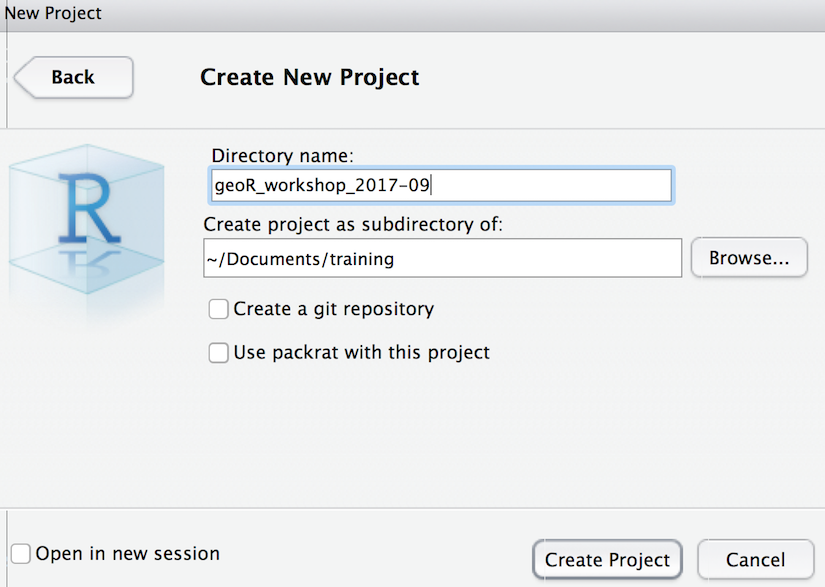
\includegraphics{figs/rstudio-new-project.png}
\caption{}
\end{figure}

\subsection{Create relative path to data
folder}\label{create-relative-path-to-data-folder}

In order to work through a common set of code and access data files in a
consistent manner, getting properly situated with paths will save many
headaches. Paths can be referenced as an ``absolute'' path starting with
your drive letter (eg ``C:'' on Windows or ``/Users'' on Mac). Absolute
paths are specific to platform (Windows / Linux / Mac) and not portable
for use on other machines or other users wishing to organize content
anywhere else. A ``relative'' path, meaning relative to your current
working directory, is portable. Try these commands in the console of
RStudio:

\begin{Shaded}
\begin{Highlighting}[]
\CommentTok{# get working directory}
\KeywordTok{getwd}\NormalTok{()}

\CommentTok{# list files in working directory}
\KeywordTok{list.files}\NormalTok{(}\StringTok{'.'}\NormalTok{)}

\CommentTok{# list files one directory up}
\KeywordTok{list.files}\NormalTok{(}\StringTok{'..'}\NormalTok{)}

\CommentTok{# create a directory}
\KeywordTok{dir.create}\NormalTok{(}\StringTok{'data'}\NormalTok{)}

\CommentTok{# set working directory}
\KeywordTok{setwd}\NormalTok{(}\StringTok{'data'}\NormalTok{)}
\KeywordTok{setwd}\NormalTok{(}\StringTok{'..'}\NormalTok{)}
\end{Highlighting}
\end{Shaded}

So you discovered the absolute path to your current working directory,
and list files in the current directory (\texttt{.}) or one directory up
(\texttt{..}). Then you created the ``data'' directory and set the
working directory to be inside of it, then back out of it.

The main reason we created the RStudio project file (filename ends in
\texttt{.Rproj}) is to have the same working directory every time you
return to this project by double-clicking the \texttt{*.Rproj} file in
your file explorer. So paths defined in the code of files there can be
based on that same working driectory and consistently work, even if you
zip them up and send to a colleague who places them on an arbitrary
location on their computer.

\section{Download data}\label{download-data}

Please download the following zip files into your newly created ``data''
folder from above.

\begin{itemize}
\tightlist
\item
  \href{https://ndownloader.figshare.com/files/3708751}{Site layout
  shapefiles}
\item
  \href{https://ndownloader.figshare.com/files/3701578}{Airborne remote
  sensing data}
\item
  \href{https://ndownloader.figshare.com/files/4933582}{Landsat NDVI
  raster data}
\item
  \href{https://ndownloader.figshare.com/files/3701572}{Meteorological
  data}
\end{itemize}

Then unzip. You should see the following when listing files (and
directories) in the data directory.

\begin{Shaded}
\begin{Highlighting}[]
\KeywordTok{list.files}\NormalTok{(}\StringTok{'data'}\NormalTok{)}
\end{Highlighting}
\end{Shaded}

\begin{verbatim}
## [1] "NEON-DS-Airborne-Remote-Sensing" "NEON-DS-Landsat-NDVI"           
## [3] "NEON-DS-Met-Time-Series"         "NEON-DS-Site-Layout-Files"      
## [5] "NEONDSAirborneRemoteSensing.zip" "NEONDSLandsatNDVI.zip"          
## [7] "NEONDSMetTimeSeries.zip"         "NEONDSSiteLayoutFiles.zip"      
## [9] "states.geojson"
\end{verbatim}

\section{Install R Packages}\label{install-r-packages}

Here's a bit of code to install packages that we'll use throughout the
workshop. Please copy and paste this code into your console.

\begin{Shaded}
\begin{Highlighting}[]
\CommentTok{# concatenate a vector of package names to install}
\NormalTok{packages =}\StringTok{ }\KeywordTok{c}\NormalTok{(}
  \CommentTok{# general data science}
  \StringTok{'tidyverse'}\NormalTok{,}
  \CommentTok{# dynamic document creation}
  \StringTok{'knitr'}\NormalTok{,}\StringTok{'rmarkdown'}\NormalTok{,}
  \CommentTok{# handle spatial data}
  \StringTok{'rgdal'}\NormalTok{,}\StringTok{'raster'}\NormalTok{,}\StringTok{'sp'}\NormalTok{,}\StringTok{'sf'}\NormalTok{,}\StringTok{'geojsonio'}\NormalTok{,}
  \CommentTok{# spatial data}
  \StringTok{'maps'}\NormalTok{,}
  \CommentTok{# spatial analysis}
  \StringTok{'rgeos'}\NormalTok{,}\StringTok{'geosphere'}\NormalTok{,}
  \CommentTok{# static plotting & mapping}
  \StringTok{'RColorBrewer'}\NormalTok{,}\StringTok{'ggplot2'}\NormalTok{,}\StringTok{'rasterVis'}\NormalTok{,}
  \CommentTok{# interactive plotting & mapping}
  \StringTok{'plotly'}\NormalTok{,}\StringTok{'leaflet'}\NormalTok{,}\StringTok{'mapview'}\NormalTok{,}\StringTok{'mapedit'}\NormalTok{)}

\CommentTok{# loop through packages}
\NormalTok{for (p in packages)\{}
  
  \CommentTok{# if package not installed}
  \NormalTok{if (!}\KeywordTok{require}\NormalTok{(p, }\DataTypeTok{character.only=}\NormalTok{T))\{}
    
    \CommentTok{# install package}
    \KeywordTok{install.packages}\NormalTok{(p)}
  \NormalTok{\}}
  
  \CommentTok{# load package}
  \KeywordTok{library}\NormalTok{(p, }\DataTypeTok{character.only=}\NormalTok{T)}
\NormalTok{\}}

\CommentTok{# report on versions of software & packages}
\KeywordTok{sessionInfo}\NormalTok{()}
\end{Highlighting}
\end{Shaded}

\begin{verbatim}
## R version 3.4.0 (2017-04-21)
## Platform: x86_64-apple-darwin15.6.0 (64-bit)
## Running under: OS X El Capitan 10.11.6
## 
## Matrix products: default
## BLAS: /Library/Frameworks/R.framework/Versions/3.4/Resources/lib/libRblas.0.dylib
## LAPACK: /Library/Frameworks/R.framework/Versions/3.4/Resources/lib/libRlapack.dylib
## 
## locale:
## [1] en_US.UTF-8/en_US.UTF-8/en_US.UTF-8/C/en_US.UTF-8/en_US.UTF-8
## 
## attached base packages:
## [1] stats     graphics  grDevices utils     datasets  methods   base     
## 
## other attached packages:
##  [1] mapedit_0.3.2       rasterVis_0.41      latticeExtra_0.6-28
##  [4] lattice_0.20-35     RColorBrewer_1.1-2  rgeos_0.3-25       
##  [7] maps_3.2.0          geojsonio_0.4.2     rgdal_1.2-11       
## [10] rmarkdown_1.6       knitr_1.17          scales_0.5.0       
## [13] htmltools_0.3.6     mapview_2.1.4       leaflet_1.1.0.9000 
## [16] plotly_4.7.1        raster_2.5-8        units_0.4-6        
## [19] geosphere_1.5-5     sp_1.2-5            bindrcpp_0.2       
## [22] sf_0.5-4            dplyr_0.7.3         purrr_0.2.3        
## [25] readr_1.1.1         tidyr_0.7.1         tibble_1.3.4       
## [28] ggplot2_2.2.1.9000  tidyverse_1.1.1    
## 
## loaded via a namespace (and not attached):
##  [1] nlme_3.1-131      satellite_1.0.0   lubridate_1.6.0  
##  [4] webshot_0.4.1     httr_1.3.1        rprojroot_1.2    
##  [7] tools_3.4.0       backports_1.1.0   R6_2.2.2         
## [10] DBI_0.7           lazyeval_0.2.0    colorspace_1.3-2 
## [13] mnormt_1.5-5      curl_2.8.1        compiler_3.4.0   
## [16] rvest_0.3.2       xml2_1.1.1        bookdown_0.5     
## [19] hexbin_1.27.1     psych_1.7.8       stringr_1.2.0    
## [22] digest_0.6.12     foreign_0.8-69    R.utils_2.5.0    
## [25] vembedr_0.1.3     base64enc_0.1-3   pkgconfig_2.0.1  
## [28] htmlwidgets_0.9   rlang_0.1.2       readxl_1.0.0     
## [31] rstudioapi_0.7    shiny_1.0.5       bindr_0.1        
## [34] zoo_1.8-0         jsonlite_1.5      crosstalk_1.0.0  
## [37] R.oo_1.21.0       magrittr_1.5      Rcpp_0.12.12     
## [40] munsell_0.4.3     R.methodsS3_1.7.1 stringi_1.1.5    
## [43] yaml_2.1.14       plyr_1.8.4        grid_3.4.0       
## [46] maptools_0.9-2    parallel_3.4.0    forcats_0.2.0    
## [49] udunits2_0.13     haven_1.1.0       hms_0.3          
## [52] gdalUtils_2.0.1.7 reshape2_1.4.2    codetools_0.2-15 
## [55] stats4_3.4.0      glue_1.1.1        evaluate_0.10.1  
## [58] V8_1.5            data.table_1.10.4 modelr_0.1.1     
## [61] png_0.1-7         httpuv_1.3.5      foreach_1.4.3    
## [64] cellranger_1.1.0  gtable_0.2.0      assertthat_0.2.0 
## [67] mime_0.5          xtable_1.8-2      broom_0.4.2      
## [70] viridisLite_0.2.0 iterators_1.0.8
\end{verbatim}

\section{Create Rmarkdown file}\label{create-rmarkdown-file}

Rmarkdown is a dynamic document format that allows you to knit chunks of
R code with formatted text (aka markdown). We recommend that you use
this format for keeping a reproducible research document as you work
through the lessons To get started, File \textgreater{} New File
\textgreater{} Rmarkdown\ldots{} and go with default HTML document and
give any title you like (default ``Untitled'' or ``test'' or ``First
Rmd'' is fine).

Check out the Help \textgreater{} Markdown Quick Reference and Help
\textgreater{} Cheatsheets \textgreater{}
\href{https://github.com/rstudio/cheatsheets/raw/master/rmarkdown-2.0.pdf}{R
Markdown Cheat Sheet}.

Here's a 1 minute video on the awesomeness of Rmarkdown:

\chapter{Tidy Spatial Analysis}\label{tidy}

\section{Overview}\label{overview}

\textbf{Questions}

\begin{itemize}
\tightlist
\item
  How to elegantly conduct complex spatial analysis by chaining
  operations?
\item
  What is the percent area of water by region across the United States?
\end{itemize}

\textbf{Objectives}

\begin{itemize}
\tightlist
\item
  Use the \texttt{\%\textgreater{}\%} operator (aka ``then'' or
  ``pipe'') to pass output from one function into input of the next.
\item
  Calculate metrics on spatial attributes.
\item
  Aggregate spatial data with metrics.
\item
  Display a map of results.
\end{itemize}

\section{Prerequisites}\label{prerequisites}

\textbf{R Skill Level}: Intermediate - you've got basics of R down.

You will use the \texttt{sf} package for vector data along with the
\texttt{dplyr} package for calculating and manipulating attribute data.

\begin{Shaded}
\begin{Highlighting}[]
\CommentTok{# load packages}
\KeywordTok{library}\NormalTok{(tidyverse)  }\CommentTok{# load dplyr, tidyr, ggplot2 packages}
\KeywordTok{library}\NormalTok{(sf)         }\CommentTok{# vector reading & analysis}

\CommentTok{# set working directory to data folder}
\CommentTok{# setwd("pathToDirHere")}
\end{Highlighting}
\end{Shaded}

\section{States: read and plot}\label{states-read-and-plot}

Similar to
\href{https://jsta.github.io/R-spatial-raster-vector-lesson/09-vector-when-data-dont-line-up-crs/}{Lesson
9: Handling Spatial Projection \& CRS in R}, we'll start by reading in a
polygon shapefile using the \texttt{sf} package. Then use the default
\texttt{plot()} function to see what it looks like.

\begin{Shaded}
\begin{Highlighting}[]
\CommentTok{# read in states}
\NormalTok{states <-}\StringTok{ }\KeywordTok{read_sf}\NormalTok{(}\StringTok{"data/NEON-DS-Site-Layout-Files/US-Boundary-Layers/US-State-Boundaries-Census-2014.shp"}\NormalTok{)}

\CommentTok{# plot the states}
\KeywordTok{plot}\NormalTok{(states)}
\end{Highlighting}
\end{Shaded}

\begin{verbatim}
## Warning: plotting the first 9 out of 10 attributes; use max.plot = 10 to
## plot all
\end{verbatim}

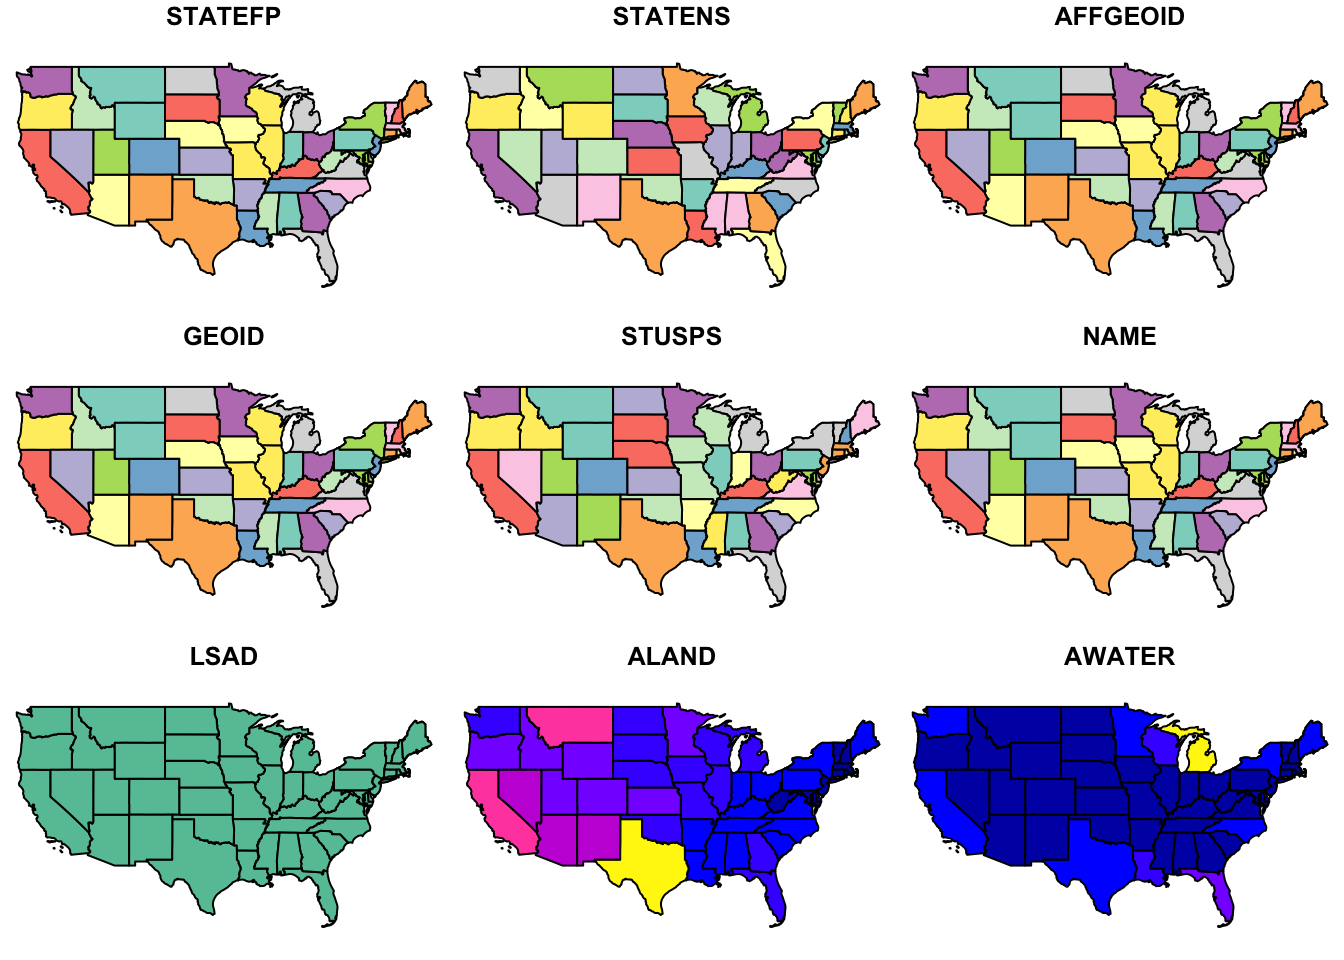
\includegraphics{R-adv-spatial_files/figure-latex/plot-states-1.pdf}

Notice the default plot on \texttt{sf} objects outputs colorized values
of the first 9 of 10 columns. Use the suggestion from the warning to
plot the 10th column.

\begin{Shaded}
\begin{Highlighting}[]
\CommentTok{# plot 10th column}
\KeywordTok{plot}\NormalTok{(states, }\DataTypeTok{max.plot =} \DecValTok{10}\NormalTok{)}
\end{Highlighting}
\end{Shaded}

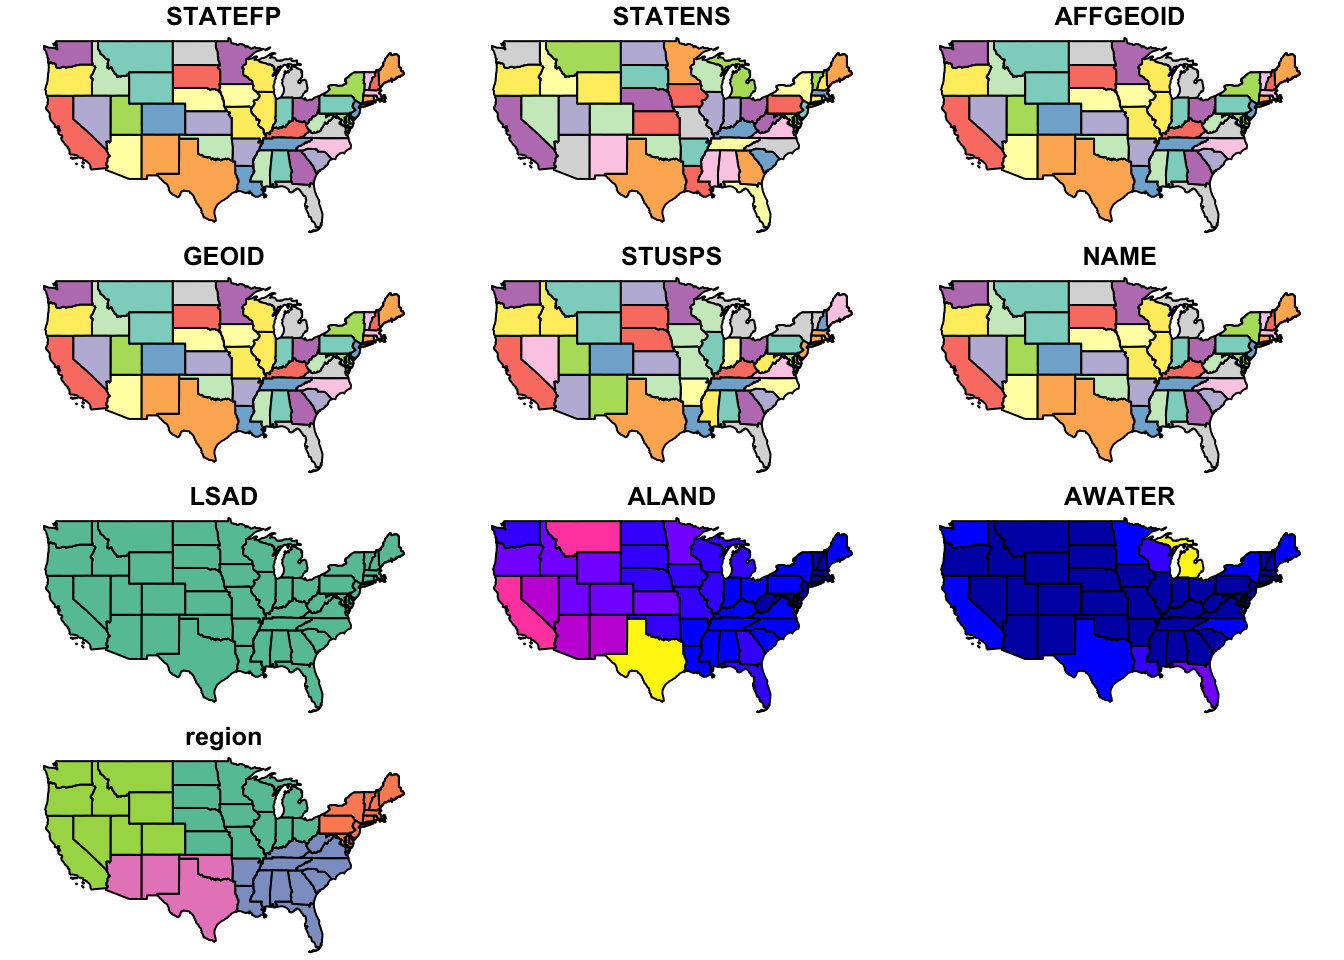
\includegraphics{R-adv-spatial_files/figure-latex/plot-states-10-1.pdf}

\begin{Shaded}
\begin{Highlighting}[]
\CommentTok{# show columns of the data frame}
\KeywordTok{names}\NormalTok{(states)}
\end{Highlighting}
\end{Shaded}

\begin{verbatim}
##  [1] "STATEFP"  "STATENS"  "AFFGEOID" "GEOID"    "STUSPS"   "NAME"    
##  [7] "LSAD"     "ALAND"    "AWATER"   "region"   "geometry"
\end{verbatim}

\begin{Shaded}
\begin{Highlighting}[]
\CommentTok{# look at table}
\KeywordTok{glimpse}\NormalTok{(states)}
\end{Highlighting}
\end{Shaded}

\begin{verbatim}
## Observations: 58
## Variables: 11
## $ STATEFP  <chr> "06", "11", "12", "13", "16", "17", "19", "21", "22",...
## $ STATENS  <chr> "01779778", "01702382", "00294478", "01705317", "0177...
## $ AFFGEOID <chr> "0400000US06", "0400000US11", "0400000US12", "0400000...
## $ GEOID    <chr> "06", "11", "12", "13", "16", "17", "19", "21", "22",...
## $ STUSPS   <chr> "CA", "DC", "FL", "GA", "ID", "IL", "IA", "KY", "LA",...
## $ NAME     <chr> "California", "District of Columbia", "Florida", "Geo...
## $ LSAD     <chr> "00", "00", "00", "00", "00", "00", "00", "00", "00",...
## $ ALAND    <dbl> 403483823181, 158350578, 138903200855, 148963503399, ...
## $ AWATER   <dbl> 20483271881, 18633500, 31407883551, 4947080103, 23977...
## $ region   <chr> "West", "Northeast", "Southeast", "Southeast", "West"...
## $ geometry <simple_feature> MULTIPOLYGONZ(((-118.593969..., MULTIPOLYG...
\end{verbatim}

\begin{Shaded}
\begin{Highlighting}[]
\CommentTok{# convert to tibble for nicer printing}
\KeywordTok{as_tibble}\NormalTok{(states)}
\end{Highlighting}
\end{Shaded}

\begin{verbatim}
## Simple feature collection with 58 features and 10 fields
## geometry type:  MULTIPOLYGON
## dimension:      XYZ
## bbox:           xmin: -124.7258 ymin: 24.49813 xmax: -66.9499 ymax: 49.38436
## epsg (SRID):    4326
## proj4string:    +proj=longlat +datum=WGS84 +no_defs
## # A tibble: 58 x 11
##    STATEFP  STATENS    AFFGEOID GEOID STUSPS                 NAME  LSAD
##      <chr>    <chr>       <chr> <chr>  <chr>                <chr> <chr>
##  1      06 01779778 0400000US06    06     CA           California    00
##  2      11 01702382 0400000US11    11     DC District of Columbia    00
##  3      12 00294478 0400000US12    12     FL              Florida    00
##  4      13 01705317 0400000US13    13     GA              Georgia    00
##  5      16 01779783 0400000US16    16     ID                Idaho    00
##  6      17 01779784 0400000US17    17     IL             Illinois    00
##  7      19 01779785 0400000US19    19     IA                 Iowa    00
##  8      21 01779786 0400000US21    21     KY             Kentucky    00
##  9      22 01629543 0400000US22    22     LA            Louisiana    00
## 10      24 01714934 0400000US24    24     MD             Maryland    00
## # ... with 48 more rows, and 4 more variables: ALAND <dbl>, AWATER <dbl>,
## #   region <chr>, geometry <simple_feature>
\end{verbatim}

\begin{Shaded}
\begin{Highlighting}[]
\KeywordTok{names}\NormalTok{(states)}
\end{Highlighting}
\end{Shaded}

\begin{verbatim}
##  [1] "STATEFP"  "STATENS"  "AFFGEOID" "GEOID"    "STUSPS"   "NAME"    
##  [7] "LSAD"     "ALAND"    "AWATER"   "region"   "geometry"
\end{verbatim}

\begin{Shaded}
\begin{Highlighting}[]
\CommentTok{# inspect the class(es) of the states object}
\KeywordTok{class}\NormalTok{(states)}
\end{Highlighting}
\end{Shaded}

\begin{verbatim}
## [1] "sf"         "tbl_df"     "tbl"        "data.frame"
\end{verbatim}

The class of the \texttt{states} object is both a simple feature
(\texttt{sf}) as well as a data frame, which means the many useful
functions available to a data frame (or ``tibble'') can be applied.

To plot the column of interest, feed the ``slice'' of that column to the
\texttt{plot()} function.

\begin{Shaded}
\begin{Highlighting}[]
\KeywordTok{plot}\NormalTok{(states[}\StringTok{'region'}\NormalTok{])}
\end{Highlighting}
\end{Shaded}

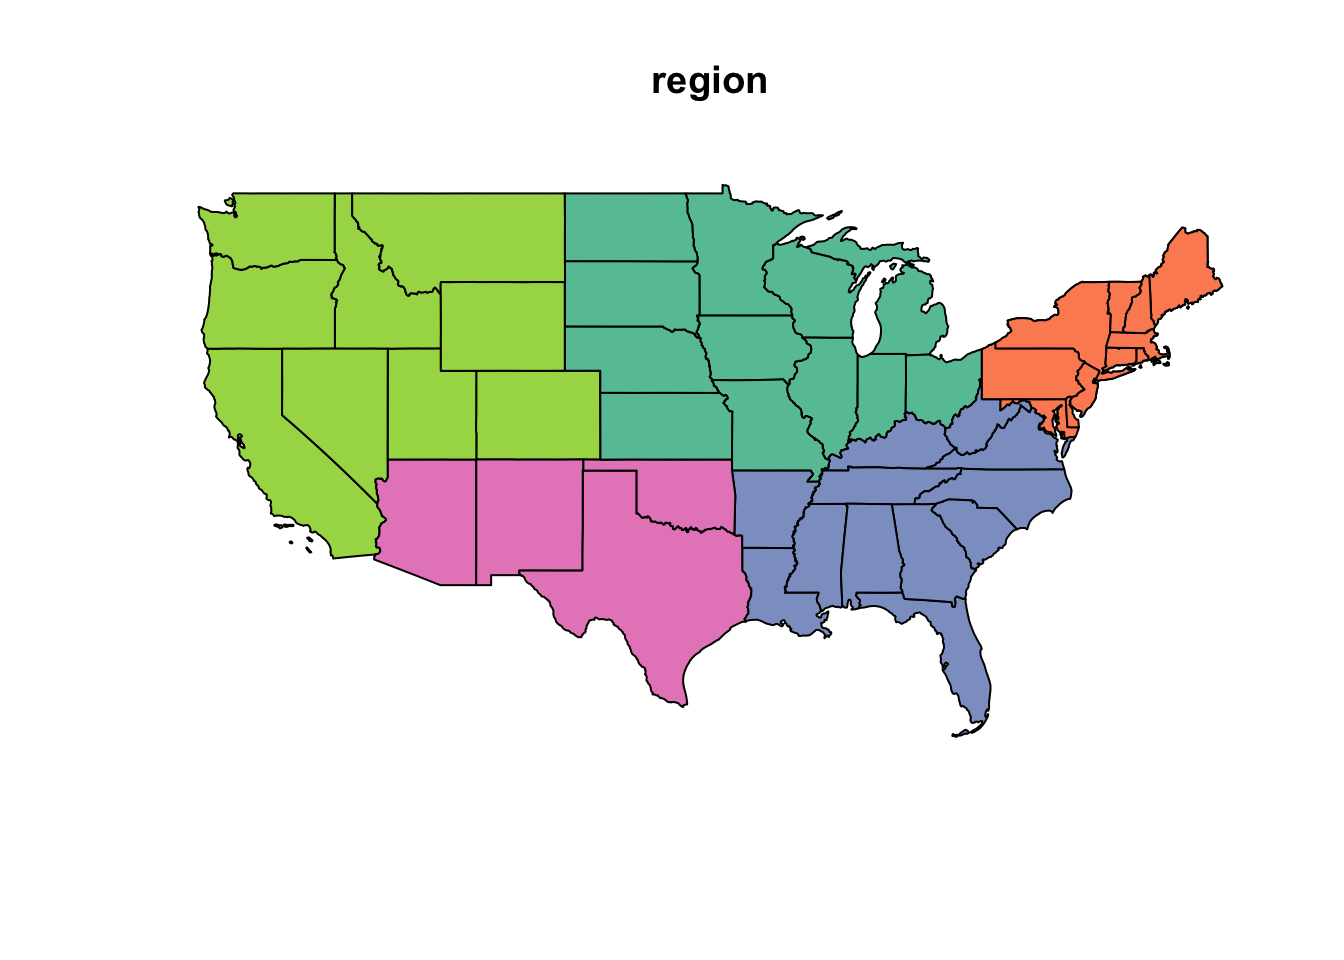
\includegraphics{R-adv-spatial_files/figure-latex/plot-states-region-1.pdf}

\textbf{Question}: To motivate the spatial analysis for the rest of this
lesson, you will answer this question: ``\emph{\textbf{What is the
percent water by region?}}''

\section{Challenge: analytical steps?}\label{challenge-analytical-steps}

Outline a sequence of analytical steps needed to arrive at the answer.

\subsection{Answers}\label{answers}

\begin{enumerate}
\def\labelenumi{\arabic{enumi}.}
\tightlist
\item
  \textbf{Sum} the area of water (\texttt{AWATER}) and land
  (\texttt{ALAND}) per region.
\item
  \textbf{Divide} the area of water (\texttt{AWATER}) by the area of
  land (\texttt{ALAND}) per region to arrive at percent water.
\item
  Show \textbf{table} of regions sorted by percent water.
\item
  Show \textbf{map} of regions by percent water with a color ramp and
  legend.
\end{enumerate}

\section{Regions: calculate \% water}\label{regions-calculate-water}

\begin{itemize}
\tightlist
\item
  Use the \texttt{\%\textgreater{}\%} operator (aka ``then'' or
  ``pipe'') to pass output from one function into input of the next.

  \begin{itemize}
  \tightlist
  \item
    In RStudio, see menu Help \textgreater{} Keyboard Shortcuts Help for
    a shortcut to the ``Insert Pipe Operator''.
  \end{itemize}
\item
  Calculate metrics on spatial attributes.

  \begin{itemize}
  \tightlist
  \item
    In RStudio, see menu Help \textgreater{} Cheatsheets \textgreater{}
    \href{https://github.com/rstudio/cheatsheets/raw/master/source/pdfs/data-transformation-cheatsheet.pdf}{Data
    Manipulation with dplyr, tidyr}.
  \end{itemize}
\item
  Aggregate spatial data with metrics.
\end{itemize}

\begin{Shaded}
\begin{Highlighting}[]
\NormalTok{regions =}\StringTok{ }\NormalTok{states %>%}
\StringTok{  }\KeywordTok{group_by}\NormalTok{(region) %>%}
\StringTok{  }\KeywordTok{summarize}\NormalTok{(}
    \DataTypeTok{water =} \KeywordTok{sum}\NormalTok{(AWATER),}
    \DataTypeTok{land  =} \KeywordTok{sum}\NormalTok{(ALAND)) %>%}
\StringTok{  }\KeywordTok{mutate}\NormalTok{(}
    \DataTypeTok{pct_water =} \NormalTok{water /}\StringTok{ }\NormalTok{land *}\StringTok{ }\DecValTok{100} \NormalTok\StringTok{ }\KeywordTok{round}\NormalTok{(}\DecValTok{2}\NormalTok{))}

\CommentTok{# object}
\NormalTok{regions}
\end{Highlighting}
\end{Shaded}

\begin{verbatim}
## Simple feature collection with 5 features and 4 fields
## geometry type:  GEOMETRY
## dimension:      XYZ
## bbox:           xmin: -124.7258 ymin: 24.49813 xmax: -66.9499 ymax: 49.38436
## epsg (SRID):    4326
## proj4string:    +proj=longlat +datum=WGS84 +no_defs
## # A tibble: 5 x 5
##      region        water         land pct_water          geometry
##       <chr>        <dbl>        <dbl>     <dbl>  <simple_feature>
## 1   Midwest 184383393833 1.943869e+12  9.485380 <MULTIPOLYGON...>
## 2 Northeast 108922434345 8.690661e+11 12.533273 <MULTIPOLYGON...>
## 3 Southeast 103876652998 1.364632e+12  7.612063 <MULTIPOLYGON...>
## 4 Southwest  24217682268 1.462632e+12  1.655761 <POLYGONZ((-9...>
## 5      West  57568049509 2.432336e+12  2.366780 <MULTIPOLYGON...>
\end{verbatim}

Notice the geometry in the column. To remove the geometry column pipe to
\texttt{st\_set\_geometry(NULL)}. To arrange in descending order use
\texttt{arrange(desc(pct\_water))}.

\begin{Shaded}
\begin{Highlighting}[]
\CommentTok{# table}
\NormalTok{regions %>%}
\StringTok{  }\KeywordTok{st_set_geometry}\NormalTok{(}\OtherTok{NULL}\NormalTok{) %>%}
\StringTok{  }\KeywordTok{arrange}\NormalTok{(}\KeywordTok{desc}\NormalTok{(pct_water))}
\end{Highlighting}
\end{Shaded}

\begin{verbatim}
## # A tibble: 5 x 4
##      region        water         land pct_water
##       <chr>        <dbl>        <dbl>     <dbl>
## 1 Northeast 108922434345 8.690661e+11 12.533273
## 2   Midwest 184383393833 1.943869e+12  9.485380
## 3 Southeast 103876652998 1.364632e+12  7.612063
## 4      West  57568049509 2.432336e+12  2.366780
## 5 Southwest  24217682268 1.462632e+12  1.655761
\end{verbatim}

\section{Regions: plot}\label{regions-plot}

Now plot the regions.

\begin{Shaded}
\begin{Highlighting}[]
\CommentTok{# plot, default}
\KeywordTok{plot}\NormalTok{(regions[}\StringTok{'pct_water'}\NormalTok{])}
\end{Highlighting}
\end{Shaded}

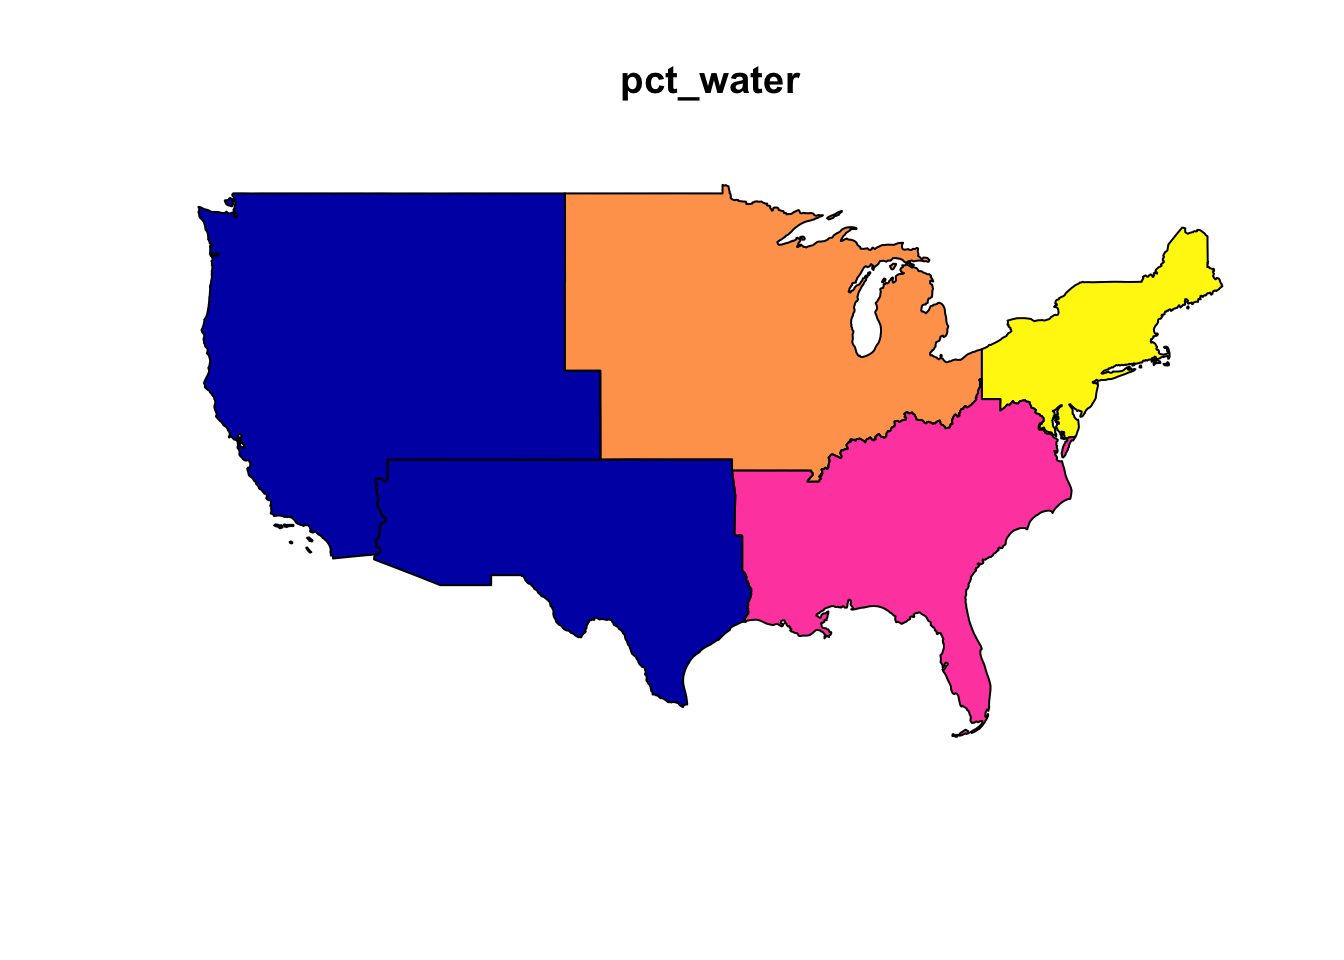
\includegraphics{R-adv-spatial_files/figure-latex/plot-regions-pctwater-1.pdf}

\section{Regions: ggplot}\label{regions-ggplot}

The \texttt{ggplot2} library can
\href{http://ggplot2.tidyverse.org/reference/ggsf.html}{visualise sf
objects}.

\begin{itemize}
\tightlist
\item
  In RStudio, see menu Help \textgreater{} Cheatsheets \textgreater{}
  \href{https://github.com/rstudio/cheatsheets/raw/master/source/pdfs/ggplot2-cheatsheet-2.1.pdf}{Data
  Visualization with ggplot2}.
\end{itemize}

\begin{Shaded}
\begin{Highlighting}[]
\CommentTok{# plot, ggplot}
\KeywordTok{ggplot}\NormalTok{(regions) +}
\StringTok{  }\KeywordTok{geom_sf}\NormalTok{(}\KeywordTok{aes}\NormalTok{(}\DataTypeTok{fill =} \NormalTok{pct_water)) +}
\StringTok{  }\KeywordTok{scale_fill_distiller}\NormalTok{(}
    \StringTok{"pct_water"}\NormalTok{, }\DataTypeTok{palette =} \StringTok{"Spectral"}\NormalTok{, }\DataTypeTok{direction=}\DecValTok{1}\NormalTok{,}
    \DataTypeTok{guide =} \KeywordTok{guide_legend}\NormalTok{(}\DataTypeTok{title =} \StringTok{"% water"}\NormalTok{, }\DataTypeTok{reverse=}\NormalTok{T)) +}
\StringTok{  }\KeywordTok{theme_bw}\NormalTok{() +}
\StringTok{  }\KeywordTok{ggtitle}\NormalTok{(}\StringTok{"% Water by US Region"}\NormalTok{)}
\end{Highlighting}
\end{Shaded}

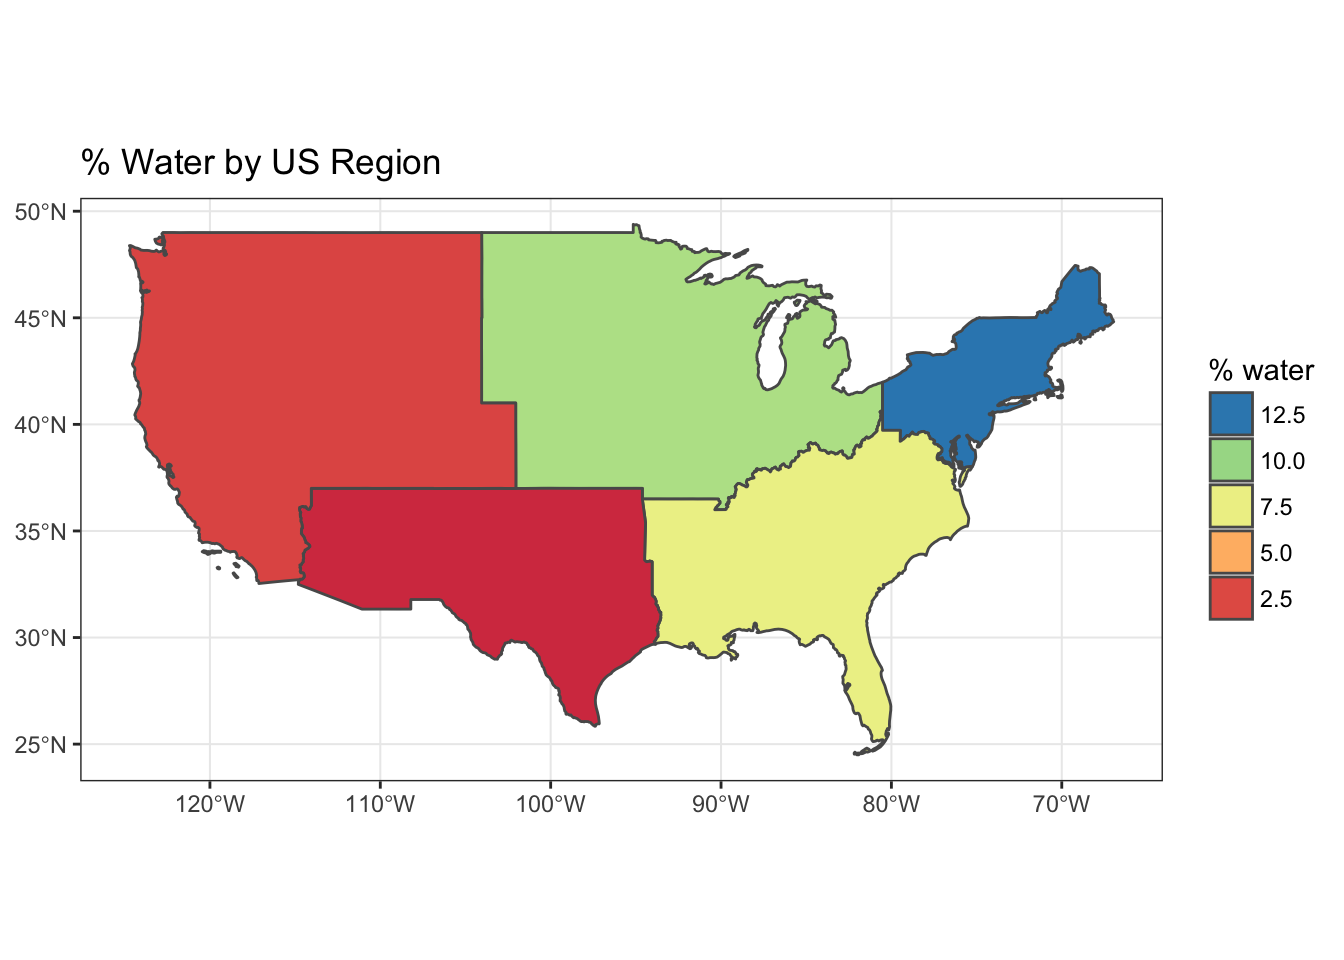
\includegraphics{R-adv-spatial_files/figure-latex/ggplot-regions-pctwater-1.pdf}

\section{Regions: recalculate area}\label{regions-recalculate-area}

So far you've used the \texttt{ALAND} column for area of the state. But
what if you were not provided the area and needed to calculate it?
Because the \texttt{states} are in geographic coordinates, you'll need
to either transform to an equal area projection and calculate area, or
use geodesic calculations. Thankfully, the \texttt{sf} library provides
area calculations with the \texttt{st\_area()} and uses the
\texttt{geosphere::distGeo()} to perform geodesic calculations (ie
trigonometric calculation accounting for the spheroid nature of the
earth). Since the \texttt{states} data has the unusual aspect of a z
dimension, you'll need to first remove that with the \texttt{st\_zm()}
function.

\begin{Shaded}
\begin{Highlighting}[]
\KeywordTok{library}\NormalTok{(geosphere)}
\KeywordTok{library}\NormalTok{(units)}

\NormalTok{regions =}\StringTok{ }\NormalTok{states %>%}
\StringTok{  }\KeywordTok{mutate}\NormalTok{(}
    \DataTypeTok{water_m2 =} \NormalTok{AWATER %>%}\StringTok{ }\KeywordTok{set_units}\NormalTok{(m^}\DecValTok{2}\NormalTok{),}
    \DataTypeTok{land_m2  =} \NormalTok{geometry %>%}\StringTok{ }\KeywordTok{st_zm}\NormalTok{() %>%}\StringTok{ }\KeywordTok{st_area}\NormalTok{()) %>%}
\StringTok{  }\KeywordTok{group_by}\NormalTok{(region) %>%}
\StringTok{  }\KeywordTok{summarize}\NormalTok{(}
    \DataTypeTok{water_m2 =} \KeywordTok{sum}\NormalTok{(water_m2),}
    \DataTypeTok{land_m2  =} \KeywordTok{sum}\NormalTok{(land_m2)) %>%}
\StringTok{  }\KeywordTok{mutate}\NormalTok{(}
    \DataTypeTok{pct_water =} \NormalTok{water_m2 /}\StringTok{ }\NormalTok{land_m2)}

\CommentTok{# table}
\NormalTok{regions %>%}
\StringTok{  }\KeywordTok{st_set_geometry}\NormalTok{(}\OtherTok{NULL}\NormalTok{) %>%}
\StringTok{  }\KeywordTok{arrange}\NormalTok{(}\KeywordTok{desc}\NormalTok{(pct_water))}
\end{Highlighting}
\end{Shaded}

\begin{verbatim}
## # A tibble: 5 x 4
##      region         water_m2          land_m2    pct_water
##       <chr>          <units>          <units>      <units>
## 1 Northeast 108922434345 m^2 9.117041e+11 m^2 0.11947126 1
## 2   Midwest 184383393833 m^2 1.987268e+12 m^2 0.09278233 1
## 3 Southeast 103876652998 m^2 1.427079e+12 m^2 0.07278971 1
## 4      West  57568049509 m^2 2.467170e+12 m^2 0.02333363 1
## 5 Southwest  24217682268 m^2 1.483765e+12 m^2 0.01632178 1
\end{verbatim}

\begin{Shaded}
\begin{Highlighting}[]
\CommentTok{# plot, ggplot}
\KeywordTok{ggplot}\NormalTok{(regions) +}
\StringTok{  }\KeywordTok{geom_sf}\NormalTok{(}\KeywordTok{aes}\NormalTok{(}\DataTypeTok{fill =} \KeywordTok{as.numeric}\NormalTok{(pct_water))) +}
\StringTok{  }\KeywordTok{scale_fill_distiller}\NormalTok{(}
    \StringTok{"pct_water"}\NormalTok{, }\DataTypeTok{palette =} \StringTok{"Spectral"}\NormalTok{, }\DataTypeTok{direction=}\DecValTok{1}\NormalTok{,}
    \DataTypeTok{guide =} \KeywordTok{guide_legend}\NormalTok{(}\DataTypeTok{title =} \StringTok{"% water"}\NormalTok{, }\DataTypeTok{reverse=}\NormalTok{T)) +}
\StringTok{  }\KeywordTok{theme_bw}\NormalTok{() +}
\StringTok{  }\KeywordTok{ggtitle}\NormalTok{(}\StringTok{"% Water by US Region"}\NormalTok{)}
\end{Highlighting}
\end{Shaded}

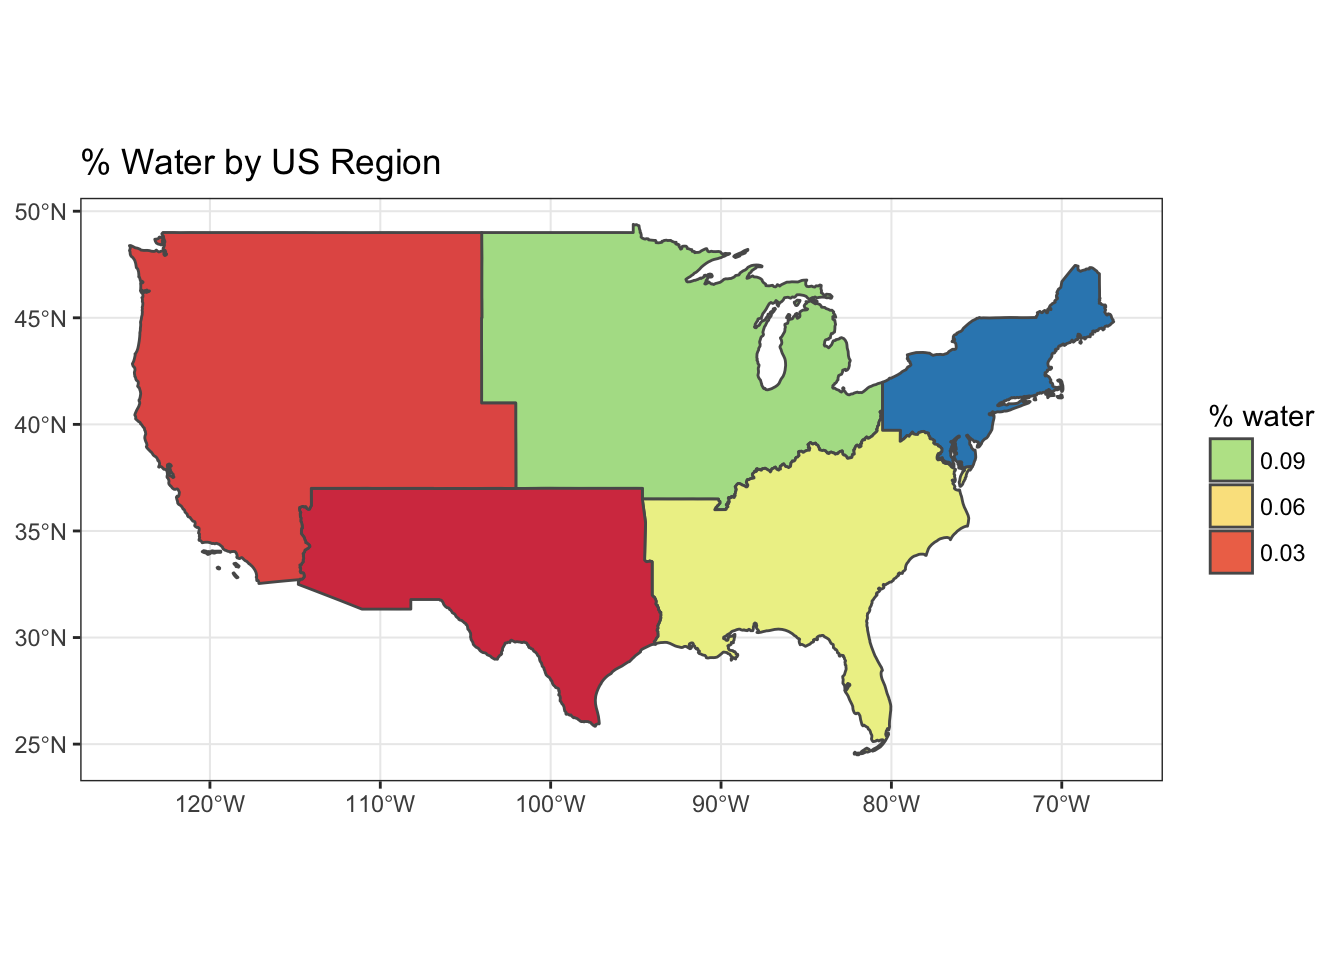
\includegraphics{R-adv-spatial_files/figure-latex/plot-regions-area-1.pdf}

\section{Challenge: project \& recalculate
area}\label{challenge-project-recalculate-area}

Use \texttt{st\_transform()} with a
\href{http://spatialreference.org/ref/esri/usa-contiguous-albers-equal-area-conic/}{USA
Contiguous Albers Equal Area Conic Projection} that minimizes
distoration, and then calculate area using the \texttt{st\_area()}
function.

\subsection{Answers}\label{answers-1}

\begin{Shaded}
\begin{Highlighting}[]
\KeywordTok{library}\NormalTok{(geosphere)}
\KeywordTok{library}\NormalTok{(units)}

\CommentTok{# Proj4 of http://spatialreference.org/ref/esri/usa-contiguous-albers-equal-area-conic/}
\NormalTok{crs_usa =}\StringTok{ '+proj=aea +lat_1=29.5 +lat_2=45.5 +lat_0=37.5 +lon_0=-96 +x_0=0 +y_0=0 +ellps=GRS80 +datum=NAD83 +units=m +no_defs'}

\NormalTok{regions =}\StringTok{ }\NormalTok{states %>%}
\StringTok{  }\KeywordTok{st_transform}\NormalTok{(crs_usa) %>%}
\StringTok{  }\KeywordTok{mutate}\NormalTok{(}
    \DataTypeTok{water_m2 =} \NormalTok{AWATER %>%}\StringTok{ }\KeywordTok{set_units}\NormalTok{(m^}\DecValTok{2}\NormalTok{),}
    \DataTypeTok{land_m2  =} \NormalTok{geometry %>%}\StringTok{ }\KeywordTok{st_zm}\NormalTok{() %>%}\StringTok{ }\KeywordTok{st_area}\NormalTok{()) %>%}
\StringTok{  }\KeywordTok{group_by}\NormalTok{(region) %>%}
\StringTok{  }\KeywordTok{summarize}\NormalTok{(}
    \DataTypeTok{water_m2 =} \KeywordTok{sum}\NormalTok{(water_m2),}
    \DataTypeTok{land_m2  =} \KeywordTok{sum}\NormalTok{(land_m2)) %>%}
\StringTok{  }\KeywordTok{mutate}\NormalTok{(}
    \DataTypeTok{pct_water =} \NormalTok{water_m2 /}\StringTok{ }\NormalTok{land_m2)}

\CommentTok{# table}
\NormalTok{regions %>%}
\StringTok{  }\KeywordTok{st_set_geometry}\NormalTok{(}\OtherTok{NULL}\NormalTok{) %>%}
\StringTok{  }\KeywordTok{arrange}\NormalTok{(}\KeywordTok{desc}\NormalTok{(pct_water))}
\end{Highlighting}
\end{Shaded}

\begin{verbatim}
## # A tibble: 5 x 4
##      region         water_m2          land_m2    pct_water
##       <chr>          <units>          <units>      <units>
## 1 Northeast 108922434345 m^2 9.117031e+11 m^2 0.11947138 1
## 2   Midwest 184383393833 m^2 1.987266e+12 m^2 0.09278246 1
## 3 Southeast 103876652998 m^2 1.427078e+12 m^2 0.07278973 1
## 4      West  57568049509 m^2 2.467167e+12 m^2 0.02333367 1
## 5 Southwest  24217682268 m^2 1.483758e+12 m^2 0.01632185 1
\end{verbatim}

\begin{Shaded}
\begin{Highlighting}[]
\CommentTok{# plot, ggplot}
\KeywordTok{ggplot}\NormalTok{(regions) +}
\StringTok{  }\KeywordTok{geom_sf}\NormalTok{(}\KeywordTok{aes}\NormalTok{(}\DataTypeTok{fill =} \KeywordTok{as.numeric}\NormalTok{(pct_water))) +}
\StringTok{  }\KeywordTok{scale_fill_distiller}\NormalTok{(}\StringTok{"pct_water"}\NormalTok{, }\DataTypeTok{palette =} \StringTok{"Spectral"}\NormalTok{) +}
\StringTok{  }\KeywordTok{theme_bw}\NormalTok{() +}
\StringTok{  }\KeywordTok{ggtitle}\NormalTok{(}\StringTok{"% Water (geodesic) by US Region"}\NormalTok{)}
\end{Highlighting}
\end{Shaded}

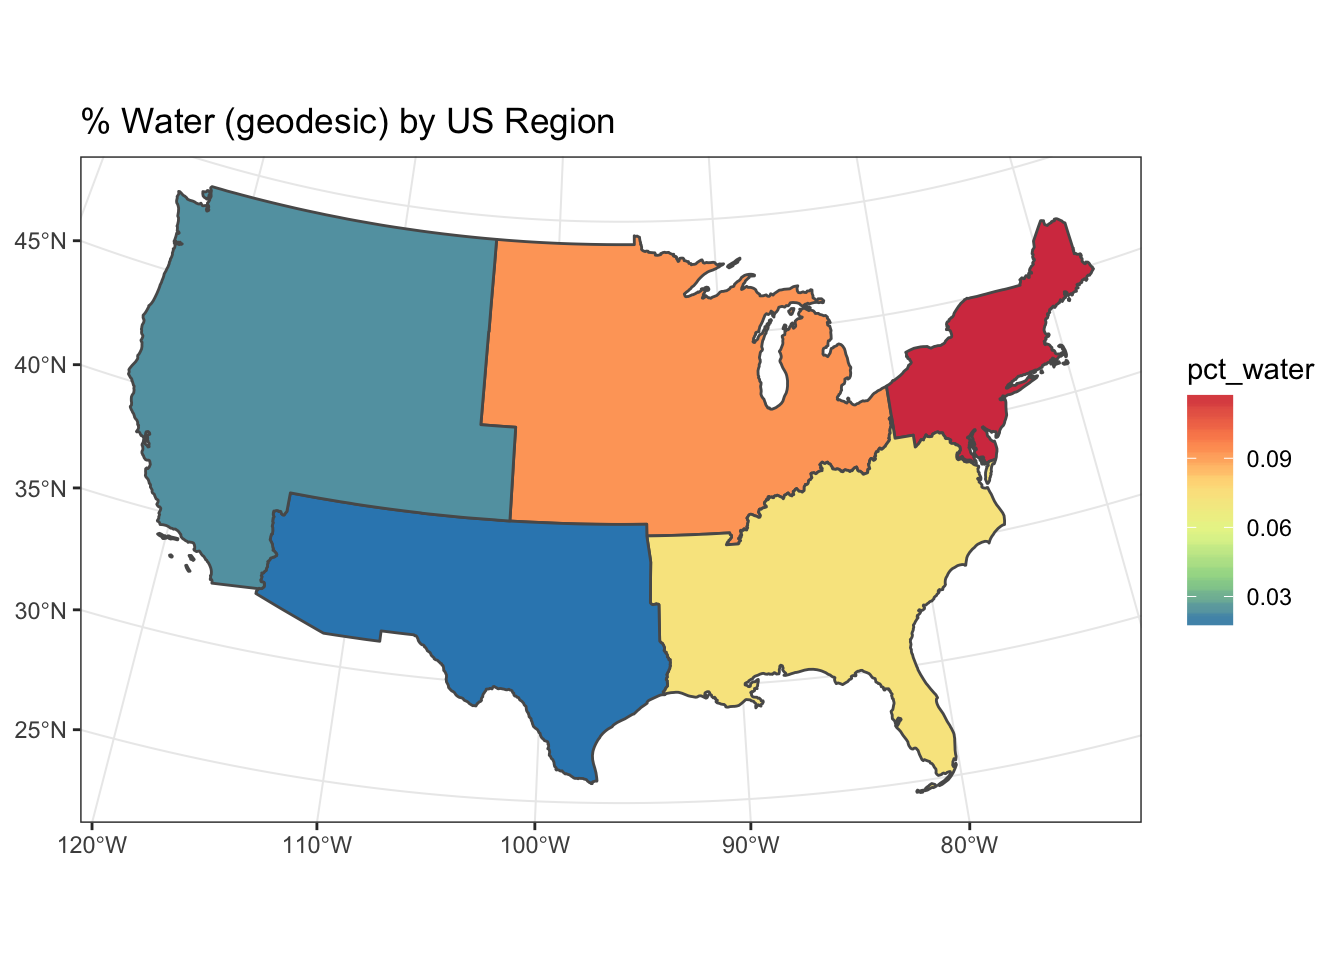
\includegraphics{R-adv-spatial_files/figure-latex/recalc-regions-transform-1.pdf}

\section{Key Points}\label{key-points}

\begin{itemize}
\tightlist
\item
  The \texttt{sf} package can take advantage of chaining spatial
  operations using the \texttt{\%\textgreater{}\%} operator.
\item
  Data manipulation functions in \texttt{dplyr} such as
  \texttt{group\_by()}, \texttt{summarize()} and \texttt{mutate()} work
  on \texttt{sf} objects.
\item
  Area can be calculated a variety of ways. Geodesic is preferred if
  starting with geographic coordinates (vs projected).
\end{itemize}

\chapter{Interactive Maps}\label{interactive}

\section{Overview}\label{overview-1}

\textbf{Questions}

\begin{itemize}
\tightlist
\item
  How do you generate interactive plots of spatial data to enable pan,
  zoom and hover/click for more detail?
\end{itemize}

\textbf{Objectives}

Learn variety of methods for producing interactive spatial output using
libraries:

\begin{itemize}
\tightlist
\item
  \texttt{plotly}: makes any ggplot2 object interactive
\item
  \texttt{mapview}: quick view of any spatial object
\item
  \texttt{leaflet}: full control over interactive map
\end{itemize}

\section{Things You'll Need to Complete this
Tutorial}\label{things-youll-need-to-complete-this-tutorial}

\textbf{R Skill Level}: Intermediate - you've got basics of R down.

We will continue to use the \texttt{sf} and \texttt{raster} packages and
introduce the \texttt{plotly}, \texttt{mapview}, and \texttt{leaflet}
packages in this tutorial.

\begin{Shaded}
\begin{Highlighting}[]
\CommentTok{# load packages}
\KeywordTok{library}\NormalTok{(tidyverse)  }\CommentTok{# loads dplyr, tidyr, ggplot2 packages}
\KeywordTok{library}\NormalTok{(sf)         }\CommentTok{# simple features package - vector}
\KeywordTok{library}\NormalTok{(raster)     }\CommentTok{# raster}
\KeywordTok{library}\NormalTok{(plotly)     }\CommentTok{# makes ggplot objects interactive}
\KeywordTok{library}\NormalTok{(mapview)    }\CommentTok{# quick interactive viewing of spatial objects}
\KeywordTok{library}\NormalTok{(leaflet)    }\CommentTok{# interactive maps}

\CommentTok{# set working directory to data folder}
\CommentTok{# setwd("pathToDirHere")}
\end{Highlighting}
\end{Shaded}

\section{States: ggplot2}\label{states-ggplot2}

Recreate the ggplot object from Lesson \ref{tidy} and save into a
variable for subsequent use with the \texttt{plotly} package.

\begin{Shaded}
\begin{Highlighting}[]
\CommentTok{# read in states}
\NormalTok{states <-}\StringTok{ }\KeywordTok{read_sf}\NormalTok{(}\StringTok{"data/NEON-DS-Site-Layout-Files/US-Boundary-Layers/US-State-Boundaries-Census-2014.shp"}\NormalTok{) %>%}
\StringTok{  }\KeywordTok{st_zm}\NormalTok{() %>%}
\StringTok{  }\KeywordTok{mutate}\NormalTok{(}
    \DataTypeTok{water_km2 =} \NormalTok{(AWATER /}\StringTok{ }\NormalTok{(}\DecValTok{1000}\NormalTok{*}\DecValTok{1000}\NormalTok{)) %>%}\StringTok{ }\KeywordTok{round}\NormalTok{(}\DecValTok{2}\NormalTok{))}

\CommentTok{# plot, ggplot}
\NormalTok{g =}\StringTok{ }\KeywordTok{ggplot}\NormalTok{(states) +}
\StringTok{  }\KeywordTok{geom_sf}\NormalTok{(}\KeywordTok{aes}\NormalTok{(}\DataTypeTok{fill =} \NormalTok{water_km2)) +}
\StringTok{  }\KeywordTok{scale_fill_distiller}\NormalTok{(}\StringTok{"water_km2"}\NormalTok{, }\DataTypeTok{palette =} \StringTok{"Spectral"}\NormalTok{) +}
\StringTok{  }\KeywordTok{ggtitle}\NormalTok{(}\StringTok{"Water (km2) by State"}\NormalTok{)}
\NormalTok{g}
\end{Highlighting}
\end{Shaded}

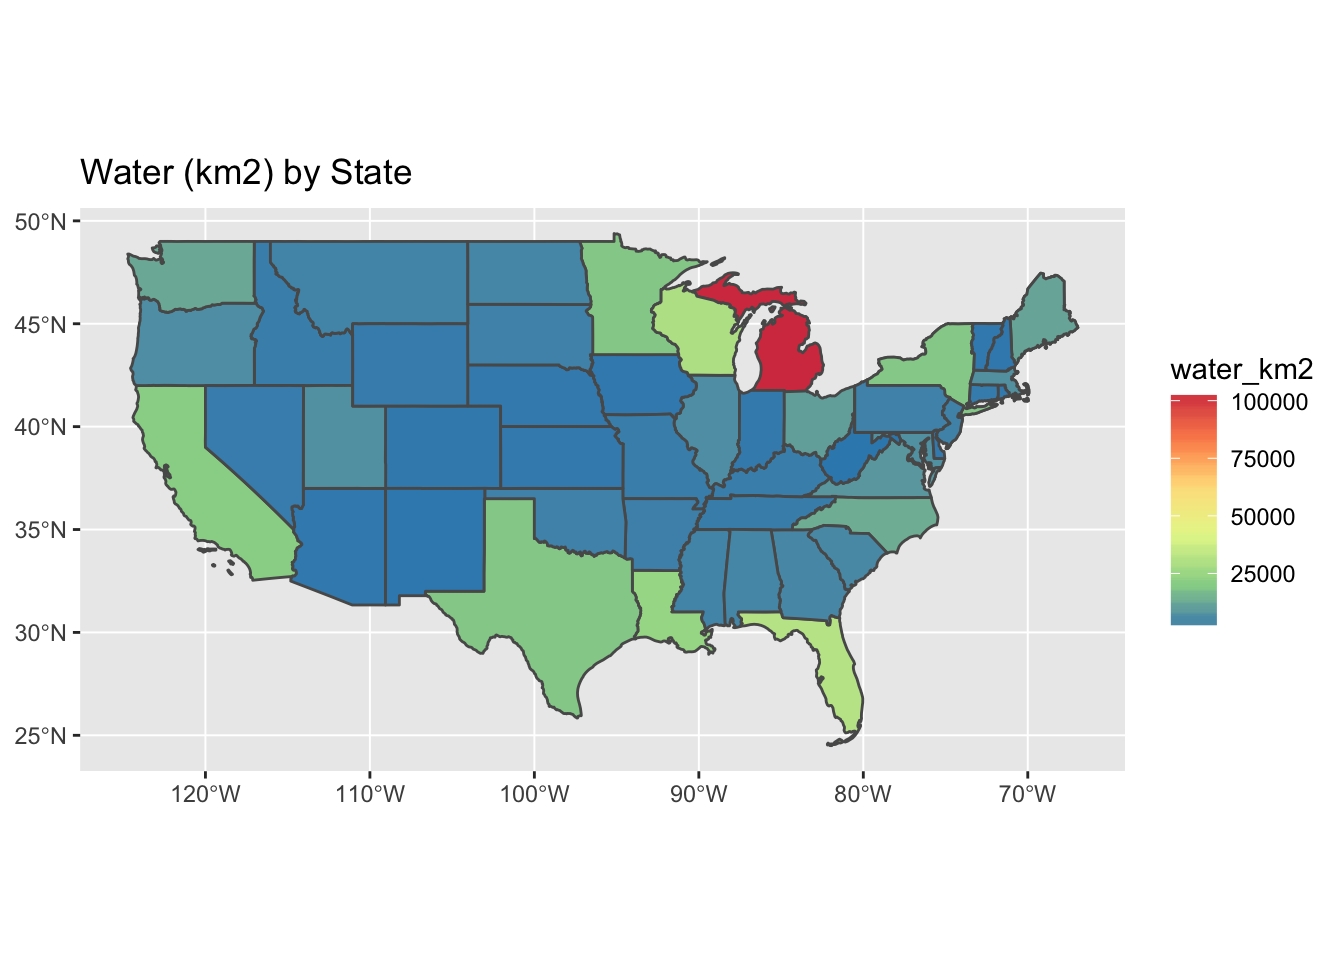
\includegraphics{R-adv-spatial_files/figure-latex/states-ggplot2-1.pdf}

\section{States: plotly}\label{states-plotly}

The \texttt{plotly::ggplotly()} function outputs a ggplot into an
interactive window capable of pan, zoom and identify.

\begin{Shaded}
\begin{Highlighting}[]
\KeywordTok{library}\NormalTok{(plotly)}

\KeywordTok{ggplotly}\NormalTok{(g)}
\end{Highlighting}
\end{Shaded}

\includegraphics{R-adv-spatial_files/figure-latex/states-plotly-1.pdf}

\section{States: mapview}\label{states-mapview}

The \texttt{mapview::mapview()} function can work for a quick view of
the data, providing choropleths, background maps and attribute popups.
Performance varies on the object and customization can be tricky.

\begin{Shaded}
\begin{Highlighting}[]
\KeywordTok{library}\NormalTok{(mapview)}

\CommentTok{# simple view with popups}
\KeywordTok{mapview}\NormalTok{(states)}
\end{Highlighting}
\end{Shaded}

\includegraphics{R-adv-spatial_files/figure-latex/states-mapview-1.pdf}

\begin{Shaded}
\begin{Highlighting}[]
\CommentTok{# coloring and layering}
\KeywordTok{mapview}\NormalTok{(states, }\DataTypeTok{zcol=}\StringTok{'water_km2'}\NormalTok{, }\DataTypeTok{burst=}\StringTok{'STUSPS'}\NormalTok{)}
\end{Highlighting}
\end{Shaded}

\includegraphics{R-adv-spatial_files/figure-latex/states-mapview-2.pdf}

\section{States: leaflet}\label{states-leaflet}

The \href{http://rstudio.github.io/leaflet/}{\texttt{leaflet}} package
offers a robust set of functions for viewing vector and raster data,
although requires more explicit functions.

\begin{Shaded}
\begin{Highlighting}[]
\KeywordTok{library}\NormalTok{(leaflet)}

\KeywordTok{leaflet}\NormalTok{(states) %>%}
\StringTok{  }\KeywordTok{addTiles}\NormalTok{() %>%}
\StringTok{  }\KeywordTok{addPolygons}\NormalTok{()}
\end{Highlighting}
\end{Shaded}

\includegraphics{R-adv-spatial_files/figure-latex/states-leaflet-1.pdf}

\subsection{Choropleth}\label{choropleth}

Drawing from the documentation from
\href{http://rstudio.github.io/leaflet/choropleths.html}{Leaflet for R -
Choropleths}, we can construct a pretty choropleth.

\begin{Shaded}
\begin{Highlighting}[]
\NormalTok{pal <-}\StringTok{ }\KeywordTok{colorBin}\NormalTok{(}\StringTok{"Blues"}\NormalTok{, }\DataTypeTok{domain =} \NormalTok{states$water_km2, }\DataTypeTok{bins =} \DecValTok{7}\NormalTok{)}


\KeywordTok{leaflet}\NormalTok{(states) %>%}
\StringTok{  }\KeywordTok{addProviderTiles}\NormalTok{(}\StringTok{"Stamen.TonerLite"}\NormalTok{) %>%}
\StringTok{  }\KeywordTok{addPolygons}\NormalTok{(}
    \CommentTok{# fill}
    \DataTypeTok{fillColor   =} \NormalTok{~}\KeywordTok{pal}\NormalTok{(water_km2),}
    \DataTypeTok{fillOpacity =} \FloatTok{0.7}\NormalTok{,}
    \CommentTok{# line}
    \DataTypeTok{dashArray   =} \StringTok{"3"}\NormalTok{,}
    \DataTypeTok{weight      =} \DecValTok{2}\NormalTok{,}
    \DataTypeTok{color       =} \StringTok{"white"}\NormalTok{,}
    \DataTypeTok{opacity     =} \DecValTok{1}\NormalTok{,}
    \CommentTok{# interaction}
    \DataTypeTok{highlight =} \KeywordTok{highlightOptions}\NormalTok{(}
      \DataTypeTok{weight =} \DecValTok{5}\NormalTok{,}
      \DataTypeTok{color =} \StringTok{"#666"}\NormalTok{,}
      \DataTypeTok{dashArray =} \StringTok{""}\NormalTok{,}
      \DataTypeTok{fillOpacity =} \FloatTok{0.7}\NormalTok{,}
      \DataTypeTok{bringToFront =} \OtherTok{TRUE}\NormalTok{))}
\end{Highlighting}
\end{Shaded}

\includegraphics{R-adv-spatial_files/figure-latex/states-choropleth-1.pdf}

\subsection{Popups and Legend}\label{popups-and-legend}

Adding a legend and popups requires a bit more work, but achieves a very
aesthetically and functionally pleasing visualization.

\begin{Shaded}
\begin{Highlighting}[]
\KeywordTok{library}\NormalTok{(htmltools)}
\KeywordTok{library}\NormalTok{(scales)}

\NormalTok{labels <-}\StringTok{ }\KeywordTok{sprintf}\NormalTok{(}
  \StringTok{"<strong>%s</strong><br/> water: %s km<sup>2</sup>"}\NormalTok{,}
  \NormalTok{states$NAME, }\KeywordTok{comma}\NormalTok{(states$water_km2)) %>%}\StringTok{ }
\StringTok{  }\KeywordTok{lapply}\NormalTok{(HTML)}

\KeywordTok{leaflet}\NormalTok{(states) %>%}
\StringTok{  }\KeywordTok{addProviderTiles}\NormalTok{(}\StringTok{"Stamen.TonerLite"}\NormalTok{) %>%}
\StringTok{  }\KeywordTok{addPolygons}\NormalTok{(}
    \CommentTok{# fill}
    \DataTypeTok{fillColor   =} \NormalTok{~}\KeywordTok{pal}\NormalTok{(water_km2),}
    \DataTypeTok{fillOpacity =} \FloatTok{0.7}\NormalTok{,}
    \CommentTok{# line}
    \DataTypeTok{dashArray   =} \StringTok{"3"}\NormalTok{,}
    \DataTypeTok{weight      =} \DecValTok{2}\NormalTok{,}
    \DataTypeTok{color       =} \StringTok{"white"}\NormalTok{,}
    \DataTypeTok{opacity     =} \DecValTok{1}\NormalTok{,}
    \CommentTok{# interaction}
    \DataTypeTok{highlight =} \KeywordTok{highlightOptions}\NormalTok{(}
      \DataTypeTok{weight =} \DecValTok{5}\NormalTok{,}
      \DataTypeTok{color =} \StringTok{"#666"}\NormalTok{,}
      \DataTypeTok{dashArray =} \StringTok{""}\NormalTok{,}
      \DataTypeTok{fillOpacity =} \FloatTok{0.7}\NormalTok{,}
      \DataTypeTok{bringToFront =} \OtherTok{TRUE}\NormalTok{),}
  \DataTypeTok{label =} \NormalTok{labels,}
  \DataTypeTok{labelOptions =} \KeywordTok{labelOptions}\NormalTok{(}
    \DataTypeTok{style =} \KeywordTok{list}\NormalTok{(}\StringTok{"font-weight"} \NormalTok{=}\StringTok{ "normal"}\NormalTok{, }\DataTypeTok{padding =} \StringTok{"3px 8px"}\NormalTok{),}
    \DataTypeTok{textsize =} \StringTok{"15px"}\NormalTok{,}
    \DataTypeTok{direction =} \StringTok{"auto"}\NormalTok{)) %>%}
\StringTok{  }\KeywordTok{addLegend}\NormalTok{(}
    \DataTypeTok{pal =} \NormalTok{pal, }\DataTypeTok{values =} \NormalTok{~water_km2, }\DataTypeTok{opacity =} \FloatTok{0.7}\NormalTok{, }\DataTypeTok{title =} \KeywordTok{HTML}\NormalTok{(}\StringTok{"Water (km<sup>2</sup>)"}\NormalTok{),}
    \DataTypeTok{position =} \StringTok{"bottomright"}\NormalTok{)}
\end{Highlighting}
\end{Shaded}

\includegraphics{R-adv-spatial_files/figure-latex/states-popups-legend-1.pdf}

\section{Challenge: leaflet for
regions}\label{challenge-leaflet-for-regions}

Use Lesson \ref{tidy} final output to create a regional choropleth with
legend and popups for percent water by region.

\subsection{Answers}\label{answers-2}

\begin{Shaded}
\begin{Highlighting}[]
\NormalTok{regions =}\StringTok{ }\NormalTok{states %>%}
\StringTok{  }\KeywordTok{group_by}\NormalTok{(region) %>%}
\StringTok{  }\KeywordTok{summarize}\NormalTok{(}
    \DataTypeTok{water =} \KeywordTok{sum}\NormalTok{(AWATER),}
    \DataTypeTok{land  =} \KeywordTok{sum}\NormalTok{(ALAND)) %>%}
\StringTok{  }\KeywordTok{mutate}\NormalTok{(}
    \DataTypeTok{pct_water =} \NormalTok{(water /}\StringTok{ }\NormalTok{land *}\StringTok{ }\DecValTok{100}\NormalTok{) %>%}\StringTok{ }\KeywordTok{round}\NormalTok{(}\DecValTok{2}\NormalTok{))}

\NormalTok{pal <-}\StringTok{ }\KeywordTok{colorBin}\NormalTok{(}\StringTok{"Spectral"}\NormalTok{, }\DataTypeTok{domain =} \NormalTok{regions$pct_water, }\DataTypeTok{bins =} \DecValTok{5}\NormalTok{)}

\NormalTok{labels <-}\StringTok{ }\KeywordTok{sprintf}\NormalTok{(}
  \StringTok{"<strong>%s</strong><br/>water: %s%%"}\NormalTok{,}
  \NormalTok{regions$region, }\KeywordTok{comma}\NormalTok{(regions$pct_water)) %>%}\StringTok{ }
\StringTok{  }\KeywordTok{lapply}\NormalTok{(HTML)}

\KeywordTok{leaflet}\NormalTok{(regions) %>%}
\StringTok{  }\KeywordTok{addProviderTiles}\NormalTok{(}\StringTok{"Stamen.TonerLite"}\NormalTok{) %>%}
\StringTok{  }\KeywordTok{addPolygons}\NormalTok{(}
    \CommentTok{# fill}
    \DataTypeTok{fillColor   =} \NormalTok{~}\KeywordTok{pal}\NormalTok{(pct_water),}
    \DataTypeTok{fillOpacity =} \FloatTok{0.7}\NormalTok{,}
    \CommentTok{# line}
    \DataTypeTok{dashArray   =} \StringTok{"3"}\NormalTok{,}
    \DataTypeTok{weight      =} \DecValTok{2}\NormalTok{,}
    \DataTypeTok{color       =} \StringTok{"white"}\NormalTok{,}
    \DataTypeTok{opacity     =} \DecValTok{1}\NormalTok{,}
    \CommentTok{# interaction}
    \DataTypeTok{highlight =} \KeywordTok{highlightOptions}\NormalTok{(}
      \DataTypeTok{weight =} \DecValTok{5}\NormalTok{,}
      \DataTypeTok{color =} \StringTok{"#666"}\NormalTok{,}
      \DataTypeTok{dashArray =} \StringTok{""}\NormalTok{,}
      \DataTypeTok{fillOpacity =} \FloatTok{0.7}\NormalTok{,}
      \DataTypeTok{bringToFront =} \OtherTok{TRUE}\NormalTok{),}
  \DataTypeTok{label =} \NormalTok{labels,}
  \DataTypeTok{labelOptions =} \KeywordTok{labelOptions}\NormalTok{(}
    \DataTypeTok{style =} \KeywordTok{list}\NormalTok{(}\StringTok{"font-weight"} \NormalTok{=}\StringTok{ "normal"}\NormalTok{, }\DataTypeTok{padding =} \StringTok{"3px 8px"}\NormalTok{),}
    \DataTypeTok{textsize =} \StringTok{"15px"}\NormalTok{,}
    \DataTypeTok{direction =} \StringTok{"auto"}\NormalTok{)) %>%}
\StringTok{  }\KeywordTok{addLegend}\NormalTok{(}
    \DataTypeTok{pal =} \NormalTok{pal, }\DataTypeTok{values =} \NormalTok{~pct_water, }\DataTypeTok{opacity =} \FloatTok{0.7}\NormalTok{, }\DataTypeTok{title =} \StringTok{"water %"}\NormalTok{,}
    \DataTypeTok{position =} \StringTok{"bottomright"}\NormalTok{)}
\end{Highlighting}
\end{Shaded}

\includegraphics{R-adv-spatial_files/figure-latex/regions-choropleth-1.pdf}

\section{Raster: leaflet}\label{raster-leaflet}

TODO: show raster overlay using NEON raster dataset example

\section{Key Points}\label{key-points-1}

\begin{itemize}
\tightlist
\item
  Interactive maps provide more detail for visual investigation,
  including use of background maps, but is only relevant in a web
  context.
\item
  Several packages exist for providing interactive views of data.
\item
  The \texttt{plotly::ggplotly()} function works quickly if you already
  have a ggplot object, which is best for static output.
\item
  The \texttt{mapview::mapview()} function can work for a quick view of
  the data, providing choropleths, background maps and attribute popups.
  Performance varies on the object and customization can be tricky.
\item
  The \texttt{leaflet} package provides a highly customizable set of
  functions for rendering of interactive choropleths with background
  maps, legends, etc.
\end{itemize}

\chapter*{References}\label{references}
\addcontentsline{toc}{chapter}{References}

\textbf{Spatial Analysis in R books}

\begin{itemize}
\tightlist
\item
  \href{http://robinlovelace.net/geocompr/}{Geocomputation with R -
  robinlovelace.net/geocompr}
\item
  \href{http://www.rspatial.org/}{Spatial Data Analysis and Modeling
  with R --- rspatial.org}
\item
  \href{http://www.spatialanalysisonline.com/HTML/index.html}{Geospatial
  Analysis 5th Edition, 2015 - spatialanalysisonline.com}
\end{itemize}

\textbf{Spatial Analysis in R blogs}

\begin{itemize}
\tightlist
\item
  \href{https://cran.r-project.org/web/views/Spatial.html}{CRAN Task
  View: Analysis of Spatial Data}
\item
  \href{http://rspatial.r-forge.r-project.org/}{R spatial projects}
\item
  \href{http://rspatial.r-forge.r-project.org/gallery/}{R sp graphics
  example figures}
\item
  \href{http://spatial.ly/r/}{Maps and Data Visualisations with R --
  spatial.ly}
\end{itemize}

\textbf{Spatial Analysis in R courses}

\begin{itemize}
\tightlist
\item
  \href{https://www.datacamp.com/courses/working-with-geospatial-data-in-r}{Spatial
  Analysis in R - datacamp.com}
\item
  \href{https://data.cdrc.ac.uk/tutorial/an-introduction-to-spatial-data-analysis-and-visualisation-in-r}{An
  Introduction to Spatial Data Analysis and Visualisation in R - CDRC
  Data}
\item
  \href{https://cengel.github.io/rspatial/}{Introduction to Mapping and
  Spatial Analysis with R - cengel.github.io/rspatial}
\item
  \href{http://geog.uoregon.edu/bartlein/courses/geog495/index.html}{GEOG
  4/595: Geographic Data Analysis - geog.uoregon.edu}
\item
  \href{http://www.maths.lancs.ac.uk/~rowlings/Teaching/UseR2012/index.html}{Geospatial
  Data in R and Beyond - maths.lancs.ac.uk}

  \begin{itemize}
  \tightlist
  \item
    \href{http://www.maths.lancs.ac.uk/~rowlings/Teaching/UseR2012/cheatsheet.html}{R
    Spatial Cheatsheet}
  \end{itemize}
\end{itemize}

\textbf{Tidy Spatial Analysis}

\begin{itemize}
\tightlist
\item
  \href{http://strimas.com/r/tidy-sf/}{Tidy spatial data in R: using
  dplyr, tidyr, and ggplot2 with sf}
\item
  \href{https://www.rstudio.com/resources/cheatsheets/}{Cheatsheets --
  RStudio}
\end{itemize}

\textbf{Interactive Maps}

\begin{itemize}
\tightlist
\item
  \href{http://remi-daigle.github.io/2016-04-15-UCSB/viz/}{Visualization
  in R - 2016-04-15-UCSB workshop}
\item
  \href{http://rstudio.github.io/leaflet/}{\texttt{leaflet}}
\item
  \href{http://r-spatial.org/r/2017/01/30/mapedit_intro.html}{\texttt{mapedit}}
\item
  \href{https://r-spatial.github.io/mapview/}{\texttt{mapview}}
\end{itemize}


\end{document}
